% ICEEICT 2027 v13: revised introduction flow with same data, metrics, and figures and verified colorized Grad-CAM.
% Colorization is deterministic from original Grayscale Grad-CAM, NOT generative art.
% Evidence-based manuscript; human authors and conference must approve before submission.
\documentclass[conference,a4paper]{IEEEtran}
\usepackage{graphicx,booktabs,array,amsmath,amssymb,cite,url}
\usepackage{tikz}
\usetikzlibrary{arrows.meta,positioning}
\usepackage[hidelinks,pdfauthor={},pdfsubject={Anonymous sewing defect detection study},pdfkeywords={broken stitch, unseen fabric, group evaluation, Grad-CAM}]{hyperref}
\begin{document}
\title{Broken-Stitch Detection on Unseen Fabrics: Group-Based Testing, Edge Fusion, and Grad-CAM Analysis}
\author{}
\maketitle
\begin{abstract}
A broken stitch can look different on different fabrics. A model that works well on familiar fabrics may fail on a new fabric. We study this problem using 3,637 normal and broken-stitch images from StitchingNet. We keep each fabric group out of training in one of five test folds. A MobileNetV3 model trained on the other fabric groups reaches 0.7969 macro-F1 with ImageNet weights and 0.8089 with added pretraining on an edited stitch-image set. However, performance changes sharply across fabric groups. We also test two ways to improve the model. Adding a small Sobel edge branch gives 0.8082 macro-F1, while training the edited-image-initialized model for 30 instead of six epochs lowers macro-F1 from 0.8075 to 0.7948 in a matched run. We use Grad-CAM to study selected cases where models make different decisions. A separate data audit shows why related augmented images must stay in the same split. Our results show that new fabric types remain a challenge. All evaluations use previously inspected data; we do not claim independent factory performance.
\end{abstract}
\begin{IEEEkeywords}
broken-stitch detection, garment inspection, unseen fabrics, group-based testing, MobileNetV3, Grad-CAM
\end{IEEEkeywords}

\section{Introduction}
Garment factories need to find broken stitches before they ship a product. A broken stitch interrupts a line of thread, but its appearance changes with fabric texture, thread color, and lighting. Some fabric patterns can also look like damaged stitches. These changes make automated inspection difficult: a model may work well on fabrics it has seen during training but make mistakes on a new fabric. We study this problem as \emph{binary broken-stitch classification on unseen fabric groups}. Given an RGB stitch image $x$ from fabric group $g$, the model predicts normal stitching ($y=0$) or a broken stitch ($y=1$). Our main goal is to measure how well it makes this decision when all images from group $g$ are excluded from training.

Earlier studies have used CNN features, image processing, and pretrained networks to detect stitch defects~\cite{kim2022,chowdhury2024,jung2025}. They show that image models can recognize many sewing defects. However, some evaluations use fabric or thread settings that also appear in training. Good scores under those conditions do not necessarily mean that a model will work well on an unseen fabric. Related augmented images can also enter different random splits and make a test score less reliable~\cite{shorten2019,kapoor2023,gerz2026}. Even when we avoid these overlaps, it is unclear whether extra pretraining, longer training, or a separate edge branch improves performance across fabrics. Overall accuracy also hides missed defects and false alarms, while an attention heatmap does not by itself confirm where a defect lies. These issues motivate an evaluation that tests both model performance and its limits.

To address this gap, we use the normal and broken-stitch classes of StitchingNet~\cite{jung2025}. We train MobileNetV3 on labeled images from some fabric groups and test it on different, held-out groups in five folds. We report macro-F1, broken-stitch recall, false alarms, and variation across fabric groups. We then compare two weight initializations and test an edge-fusion branch and a longer training schedule under matched settings. We also inspect selected model decisions with Grad-CAM and examine how related-image splitting affects a separate edited-image dataset. \emph{Our positioning is an evaluation and failure-analysis study}, not a claim of a new architecture or a state-of-the-art detector. Because our models learn from other StitchingNet fabrics, our tests measure unseen-fabric generalization within this dataset, not zero-shot transfer to an independent factory.

These goals lead to four research questions:
\begin{enumerate}
\item[\textbf{RQ1:}] How does performance change across held-out fabric groups, and how do related-image splits affect a separate development evaluation?
\item[\textbf{RQ2:}] Does additional pretraining on edited stitch images improve fabric-held-out macro-F1 compared with ImageNet initialization alone?
\item[\textbf{RQ3:}] Does extending training from six to 30 epochs or adding a Sobel edge branch improve performance on the same held-out fabrics?
\item[\textbf{RQ4:}] What do Grad-CAM maps show in selected correct and missed detections, and what are the limits of those explanations?
\end{enumerate}
We answer these questions through four contributions. First, we report five-fold fabric-held-out results with class-specific error counts. Second, we compare initializations, training duration, and edge fusion using matched fabric folds. Third, we audit augmentation-family overlap and compare image-random with photo-grouped development splits. Finally, we examine the same broken-stitch cases with two trained models and report what Grad-CAM can and cannot explain. Together, these experiments identify practical limits of broken-stitch classification without claiming independent factory validation.

\section{Related Work}
\subsection{Stitch detection and industrial image models}
Kim \emph{et al.}~\cite{kim2022} used CNN features and image processing to find broken stitches. Chowdhury \emph{et al.}~\cite{chowdhury2024} compared CNN, VGG-16, and VGG-19 models on a small stitch-image dataset. Jung \emph{et al.}~\cite{jung2025} introduced StitchingNet and tested transfer learning on normal stitches and ten defect classes. Their test split included images from fabric settings also present in training. Our test folds instead leave out whole fabric settings. As a result, the scores from these studies do not form a direct ranking. More recent work studied sewing defects with PatchCore~\cite{kimpatch2026} and released StitchingNet-Seg masks~\cite{parkseg2026}. StitchingNet-Seg comes from StitchingNet, so it cannot serve as a new independent test of the same images.

Researchers have also studied defects in other industrial images. MVTec AD offers real anomaly images and pixel labels~\cite{bergmann2019}. DRAEM uses simulated defects to learn anomaly features~\cite{draem2021}. PatchCore uses stored image patches to find unusual regions~\cite{roth2022}. These methods provide useful ideas, but their data and labels differ from broken sewing stitches. We therefore focus on direct normal-versus-broken classification under a fixed fabric-group test.

\subsection{Data shifts, model design, and explanations}
Training and test data can differ even when they come from the same industry. Work on domain generalization shows why groups and test conditions matter~\cite{zhou2023,koh2021,gulrajani2021,sagawa2020}. We use complete fabric groups as our test unit. We do not assume that different fabrics also mean independent cameras or factories.

MobileNetV3 offers a small pretrained image model and already uses channel attention~\cite{howard2019,hu2018}. We test a second branch that extracts image edges, but we treat it as an experiment rather than a new kind of network. For explanations, Grad-CAM highlights image areas that influence a chosen model score~\cite{selvaraju2017}. Saliency tests also warn that a plausible heatmap may not give a trustworthy explanation~\cite{adebayo2018}. We use heatmaps to describe selected cases, not to score the location of defects.

\begin{table}[!t]\centering
\caption{How this study differs from earlier sewing-defect work. Results from different tasks and test splits should not be compared as one ranking.}\label{tab:prior}
\footnotesize\setlength{\tabcolsep}{3.2pt}
\begin{tabular}{p{.23\columnwidth}p{.34\columnwidth}p{.31\columnwidth}}\toprule
Study & Main method & Main test setting\\\midrule
Kim \emph{et al.}~\cite{kim2022} & CNN features and image processing & Broken-stitch images\\
Chowdhury \emph{et al.}~\cite{chowdhury2024} & CNN and VGG models & Small binary dataset\\
Jung \emph{et al.}~\cite{jung2025} & CNN and transformer transfer learning & Split within each fabric setting\\
Our study & MobileNetV3, extra edge branch, Grad-CAM & Hold out entire fabric groups\\\bottomrule
\end{tabular}
\end{table}

\section{Data and Methods}
\subsection{Datasets}
We use two sets of stitch images. The first contains 7,364 readable images of normal stitches and digitally edited defects. Many images come from the same starting photo through editing or augmentation. File names suggest 31 photo groups, but we cannot confirm these groups from original camera records. We use this set to test data splits and to prepare one set of initial model weights. We never treat its edited defects as proof of performance on real broken stitches.

Our main test uses StitchingNet~\cite{jung2025}. We select only class 00 (2,436 normal stitches) and class 02 (1,201 broken stitches). These 3,637 images cover eleven fabric and thread settings, A--K. We do not use the other defect classes in this binary experiment. Table~\ref{tab:data} summarizes the two sets.

\begin{table}[!t]\centering
\caption{Datasets used in the experiments. The edited-image set has more image files than independently verified source photos.}\label{tab:data}
\footnotesize\setlength{\tabcolsep}{3pt}
\begin{tabular}{p{.43\columnwidth}rr}\toprule
Dataset & Images & Groups\\\midrule
Edited stitch-image set & 7,364 & 31 suggested photo groups\\
StitchingNet normal/broken & 3,637 & 11 fabric settings\\\bottomrule
\end{tabular}
\end{table}

\subsection{Check for related images across splits}
We use image file names to find repeated augmentation families. We then check whether members of the same family appear in different dataset folders. We also compare exact file hashes. For a second check, we join edited defects with their suggested starting photos. We use these photo groups to keep related images together. Because we do not have the original editing logs, the group identities remain estimates.

We compare two five-fold tests on 6,278 development images from 26 suggested photo groups. The first test splits images at random. The second keeps each photo group in one fold. Both use the same frozen MobileNetV3 image features and the same balanced logistic classifier. Only the split rule changes. This is an exploratory check of how test design changes the score; it is not an estimate of performance in a new factory.

\subsection{Test on unseen fabrics}
We split the eleven StitchingNet fabric settings into five folds. For each fold, we train on the other fabrics and test on the held-out fabrics. We check that no fabric ID appears on both sides. We combine the five test predictions only after training ends. We use the same folds for all matching models.

We train MobileNetV3-Small in two ways. Model A starts from ImageNet weights. Model B starts from ImageNet weights and then uses weights learned from the edited stitch-image set. \emph{Both models train on labeled StitchingNet images from the other fabrics.} They are not tests of a model that has never seen real stitch labels. We also evaluate a separate model trained only on the edited images, but we keep its results apart because the training data differ.

Both fabric-trained models use 224$\times$224 input images, a batch size of 16, six epochs, AdamW, and class-weighted binary cross-entropy. The classifier head uses a learning rate of $5\times10^{-4}$, and the trainable last feature layers use $10^{-4}$. Weight decay is $10^{-4}$. During training, we rotate images by up to $8^{\circ}$ and make small brightness and contrast changes. We keep batch-normalization statistics fixed. Test fabrics never update model weights or set the decision threshold.

\subsection{Longer training and an extra edge branch}
We first test whether six epochs are enough. We keep the same training setup and continue a separate matched run to 30 epochs. We record predictions at epochs 6 and 30. We choose these points before looking at their results. This lets us compare training time without changing the test fabrics.

Next, we add a small edge branch to the six-epoch MobileNetV3 model. A Sobel filter finds strong brightness changes. Two small convolutional layers learn features from this edge map. The branch produces one score. A learned gate combines this score with MobileNetV3's score:
\begin{equation}
 z(x)=z_{\mathrm{MobileNet}}(x)+\tanh(g)z_{\mathrm{edge}}(x),\qquad g=0\ \text{at start}.
\label{eq:fusion}
\end{equation}
The zero gate makes the new model start with the same prediction as MobileNetV3. Training can then raise or lower the edge branch's effect. This model combines \emph{two scores}; it does not segment the broken thread. Figure~\ref{fig:fusion} shows the design.

\begin{figure}[!t]\centering
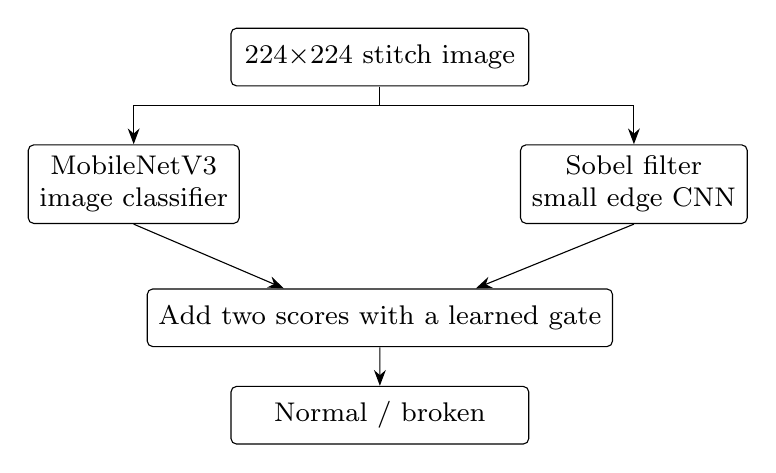
\begin{tikzpicture}[scale=1.22,transform shape,font=\footnotesize, node distance=3.5mm,
 node/.style={draw,rounded corners=2pt,align=center,minimum height=6mm},
 >={Stealth[length=2mm]}]
\node[node,minimum width=3.1cm] (image) {224$\times$224 stitch image};
\node[node,below left=6mm and -1mm of image,minimum width=2.05cm] (cnn) {MobileNetV3\\image classifier};
\node[node,below right=6mm and -1mm of image,minimum width=2.05cm] (edge) {Sobel filter\\small edge CNN};
\node[node,below=21mm of image,minimum width=3.1cm] (fusion) {Add two scores with a learned gate};
\node[node,below=4mm of fusion,minimum width=3.1cm] (out) {Normal / broken};
\draw[->] (image.south) -- ++(0,-2mm) -| (cnn.north);
\draw[->] (image.south) -- ++(0,-2mm) -| (edge.north);
\draw[->] (cnn.south) -- ([xshift=-10mm]fusion.north);
\draw[->] (edge.south) -- ([xshift=10mm]fusion.north);
\draw[->] (fusion) -- (out);
\end{tikzpicture}
\caption{Input/output view of our edge-fusion test model. It takes a stitch image and predicts normal or broken. A learned gate adds the edge branch's score to the MobileNetV3 score. We compare it with the unchanged MobileNetV3 model on the same held-out fabrics.}\label{fig:fusion}
\end{figure}

\subsection{How we measure and explain errors}
We use macro-F1 as the main score and set the decision threshold to 0.5. We also count missed broken stitches and false alarms on normal stitches. We report balanced accuracy, broken-stitch recall, and results for each fabric fold. For matched models, we resample the eleven fabric groups to describe uncertainty. Eleven groups from one collection cannot prove that a change will help in other factories.

We use Grad-CAM to inspect ten real broken-stitch images. We select one correct broken-stitch detection and one missed broken stitch from each held-out fold of the fabric-trained model. We then compare the two model scores and heatmaps on each selected image. We also replace the strongest and weakest 20\% of the edited-image-only model's highlighted areas with average-color pixels and record the change in score. The final feature maps have only $7\times7$ cells before resizing. The ten chosen examples are not a random sample. We therefore do not use them to estimate overall recall or to claim accurate defect location~\cite{selvaraju2017,adebayo2018}.

\section{Results and Discussion}
\subsection{Why the test split matters}
All 182 detected augmentation families appear in more than one original folder, although file hashes do not show identical copies across those folders. The file names also link 151 edited-defect families to 31 suggested starting photos. We cannot confirm those photo links without editing records.

On 6,278 development images, the random-image test reaches 0.8714 macro-F1. The photo-group test reaches 0.6879. This 0.1835 difference shows that the split choice has a large effect in this dataset. It does not measure how much any earlier model's score was overstated, because the groups and images in the folds also differ.

\subsection{Performance on unseen fabrics}
Table~\ref{tab:perf} gives the results for the 3,637 StitchingNet images. The model trained only on edited stitch images reaches 0.7253 macro-F1 in a separate, already-inspected transfer test. In the main held-out-fabric test, ImageNet-started MobileNetV3 reaches 0.7969. The model with extra edited-image pretraining reaches 0.8089. This change is small. The 11-fabric bootstrap interval for the difference is $[-0.0090,0.0360]$, which includes zero. We therefore cannot claim that extra pretraining gives a reliable gain.

\begin{table}[!t]\centering
\caption{Results on StitchingNet (3,637 images; threshold 0.5). The first row uses no StitchingNet training; do not compare it as a matched model. The six- and 30-epoch rows come from the same new training runs. FP: false alarms; FN: missed broken stitches.}\label{tab:perf}
\footnotesize\setlength{\tabcolsep}{2.5pt}
\begin{tabular}{p{.45\columnwidth}rrrr}\toprule
Training setup & F1 & Recall & FP & FN\\\midrule
Edited images only & .7253 & .7194 & 589 & 337\\
ImageNet + real fabrics, 6e & .7969 & .9301 & 628 & 84\\
Edited-init. + real fabrics, 6e & \textbf{.8089} & .9134 & 559 & 104\\
MobileNet + edge branch, 6e & .8082 & .9142 & 563 & 103\\\midrule
New run: ImageNet, 6e & .7951 & .9267 & 630 & 88\\
New run: ImageNet, 30e & .7652 & .9700 & 804 & 36\\
New run: edited-init., 6e & .8075 & .9159 & 568 & 101\\
New run: edited-init., 30e & .7948 & .9409 & 651 & 71\\\bottomrule
\end{tabular}
\end{table}

The fabric-trained model with extra edited-image pretraining reaches 0.9634 macro-F1 on fabrics B/F but only 0.6931 on fabrics I/J. Other folds lie between these values. Figure~\ref{fig:folds} shows this gap. The model does not work equally well on every new fabric group.

\begin{figure}[!t]\centering
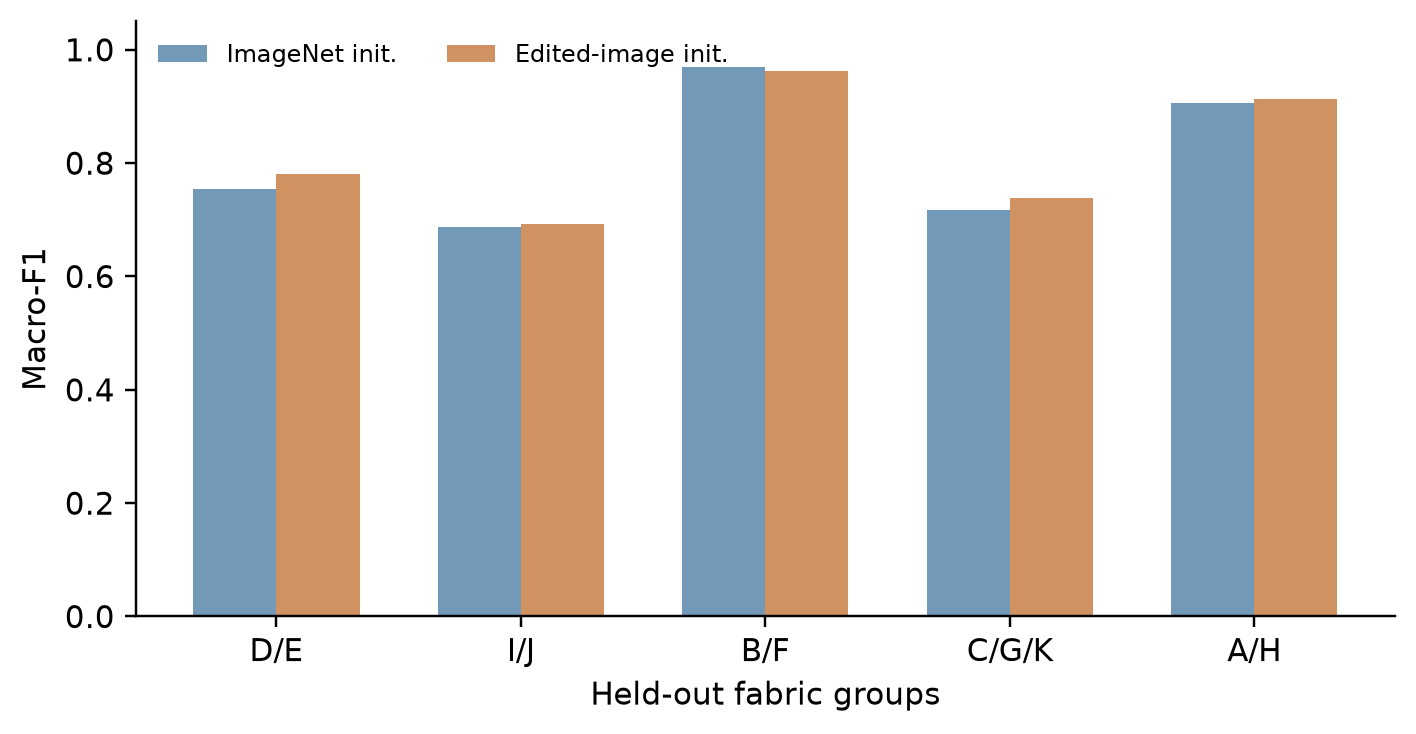
\includegraphics[width=\columnwidth]{figures_v13/heldout_fabric_macro_f1.png}
\caption{Macro-F1 for each held-out fabric fold. Each fold tests fabrics that the model did not see during training. Fabric groups vary widely in difficulty.}\label{fig:folds}
\end{figure}

\subsection{Do more epochs or extra edges help?}
Training for 30 epochs does not raise macro-F1 at the fixed threshold. In the ImageNet-started run, macro-F1 falls from 0.7951 to 0.7652. In the edited-image-started run, it falls from 0.8075 to 0.7948. Longer training finds more broken stitches, but it also creates more false alarms. For example, the latter run cuts missed broken stitches from 101 to 71 while false alarms rise from 568 to 651. The paired fabric-group intervals include zero, so we do not treat the difference as a proven drop in all future settings.

The added edge branch also fails to improve macro-F1. It reaches 0.8082, compared with 0.8089 for the matched MobileNetV3 baseline. It misses 103 broken stitches instead of 104 but raises false alarms from 559 to 563. The small change does not support a claim that this hybrid model works better on new fabrics.

\subsection{What Grad-CAM shows}
Table~\ref{tab:xai} shows five examples from our ten selected real broken-stitch images. For examples from fabrics D, C, and A, the model trained only on edited images misses the defect, while the model trained on other real fabrics detects it. The opposite happens for the selected fabric B image. On fabric J, both models miss the defect. These examples show disagreements. They do not explain the exact reason for each decision.

\begin{table}[!t]\centering
\caption{Selected broken-stitch images. Values show the model's broken-stitch probability. We chose these cases after observing results, so they cannot estimate dataset-wide recall.}\label{tab:xai}
\footnotesize\setlength{\tabcolsep}{3.7pt}
\begin{tabular}{lrr}\toprule
Fabric & Edited-only model & Fabric-trained model\\\midrule
D & .053 & .664\\
C & .034 & .942\\
A & .165 & .998\\
B & .988 & .259\\
J & .007 & .044\\\bottomrule
\end{tabular}
\end{table}

\begin{figure}[!t]\centering
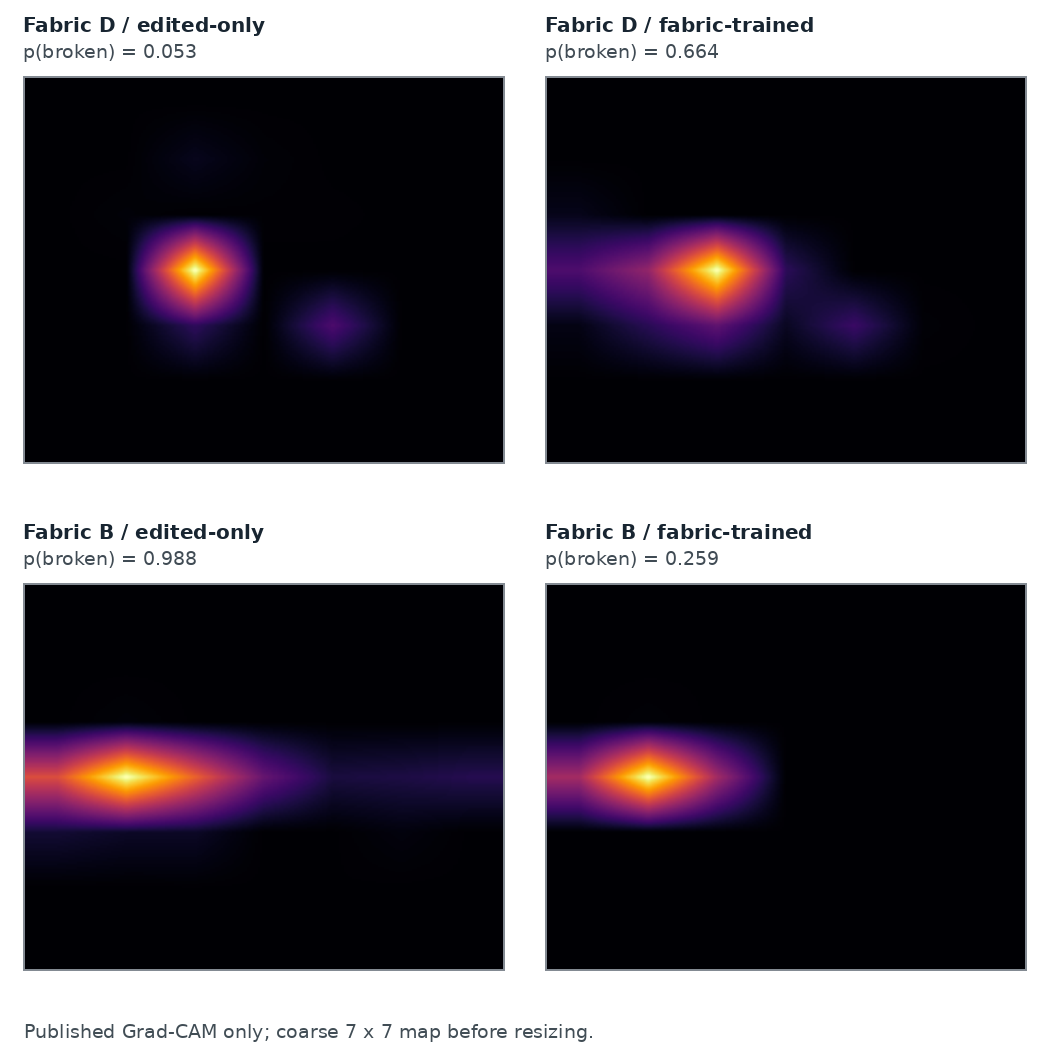
\includegraphics[width=\columnwidth]{figures_v13/verified_cam_colorized_D_B.png}
\caption{Verified Grad-CAM on two selected broken-stitch cases. Each row compares the same image using an edited-image-only model (left) and a fabric-trained model (right). We apply a fixed, monotonic false-color map to the saved grayscale CAMs. The model features have only $7\times7$ spatial cells. We do not claim accurate defect localization.} \label{fig:xai}
\end{figure}

We use the same fixed color conversion for the four published grayscale maps. Each map was normalized separately when created, so their colors are not comparable as absolute activation values. The Grad-CAM maps highlight different areas for the two models, but each map uses its own scale. We cannot compare their brightness directly. We also have no expert defect masks for these examples. Thus, the maps help us discuss individual failures, not prove which pixels caused them. The original experiment files provide the per-image scores and heatmaps.\footnote{\href{https://github.com/kahakashanashraf/Broken-Stitch-Detection-in-Garment-Manufacturing/releases/tag/thesis-only-vs-fabric-heldout-gradcam-v1}{Public Grad-CAM images and case data (GitHub release)}.}

\section{Limitations and Conclusion}
We test only eleven fabric settings from one source. Different settings may still share cameras, machines, or capture sessions. The data have already been examined during model development, so our results are exploratory rather than a fresh blind test. We cannot confirm the original photo groups in the edited-image set from source records. The selected Grad-CAM cases are too few and too carefully chosen to measure explanation quality. We also lack expert defect masks and new test images from independent factories.

Our study finds that held-out-fabric performance varies widely. A MobileNetV3 model trained on other real fabrics reaches 0.8089 macro-F1, but stronger training and an added Sobel edge branch do not raise this score in our matched tests. The data audit shows why related images should not cross splits. Grad-CAM helps us inspect selected mistakes, but it does not prove where a defect lies. Future work should collect independently captured fabrics and compare stronger models using the same fixed group-based test.

\section*{Generative-AI Use Disclosure}
AI tools helped with research planning, code workflows, literature searches, and writing. The human authors must check and approve every claim, reference, figure, and data permission. The conference must confirm that this use meets its policy before submission.

\begin{thebibliography}{00}\footnotesize
\bibitem{ngan2011} H. Y. T. Ngan, G. K. H. Pang, and N. H. C. Yung, ``Automated fabric defect detection---A review,'' \emph{Image Vis. Comput.}, vol. 29, no. 7, pp. 442--458, 2011, doi: 10.1016/j.imavis.2011.02.002.
\bibitem{kim2022} H. Kim, W.-K. Jung, Y.-C. Park, J.-W. Lee, and S.-H. Ahn, ``Broken stitch detection method for sewing operation using CNN feature map and image-processing techniques,'' \emph{Expert Syst. Appl.}, vol. 188, art. 116014, 2022, doi: 10.1016/j.eswa.2021.116014.
\bibitem{chowdhury2024} H. Chowdhury \emph{et al.}, ``Broken stitch detection method for sewing operation using deep learning,'' in \emph{Proc. Int. Conf. Innovations in Science, Engineering and Technology (ICISET)}, 2024, doi: 10.1109/ICISET62123.2024.10939324.
\bibitem{jung2025} W.-K. Jung, J. Kang, W. Kwon, and H. Kim, ``StitchingNet and deep transfer learning method for sewing stitch defect detection,'' \emph{J. Comput. Des. Eng.}, vol. 12, no. 4, pp. 140--154, 2025, doi: 10.1093/jcde/qwaf037.
\bibitem{shorten2019} C. Shorten and T. M. Khoshgoftaar, ``A survey on image data augmentation for deep learning,'' \emph{J. Big Data}, vol. 6, art. 60, 2019, doi: 10.1186/s40537-019-0197-0.
\bibitem{kapoor2023} S. Kapoor and A. Narayanan, ``Leakage and the reproducibility crisis in machine-learning-based science,'' \emph{Patterns}, vol. 4, no. 9, art. 100804, 2023, doi: 10.1016/j.patter.2023.100804.
\bibitem{gerz2026} F. Gerz and M. Jelali, ``Towards reliable data augmentation in machine learning: Practices to prevent data leakage,'' \emph{Smart Agric. Technol.}, vol. 15, art. 102462, 2026, doi: 10.1016/j.atech.2026.102462.
\bibitem{zhou2023} K. Zhou, Z. Liu, Y. Qiao, T. Xiang, and C. C. Loy, ``Domain generalization: A survey,'' \emph{IEEE Trans. Pattern Anal. Mach. Intell.}, vol. 45, no. 4, pp. 4396--4415, 2023, doi: 10.1109/TPAMI.2022.3195549.
\bibitem{koh2021} P. W. Koh \emph{et al.}, ``WILDS: A benchmark of in-the-wild distribution shifts,'' in \emph{Proc. Int. Conf. Mach. Learn.}, PMLR 139, 2021, pp. 5637--5664.
\bibitem{kimpatch2026} J. Kim, J.-H. Woo, W.-K. Jung, and H. Kim, ``An efficient anomaly detection method for the industrial sewing process using PatchCore and fine-tuned ResNet,'' \emph{Sci. Rep.}, 2026, doi: 10.1038/s41598-026-73203-5.
\bibitem{parkseg2026} J. Park, W.-K. Jung, and H. Kim, ``StitchingNet-Seg: A semantic segmentation dataset of industrial sewing stitch defects,'' \emph{Sci. Data}, 2026, doi: 10.1038/s41597-026-08496-2.
\bibitem{bergmann2019} P. Bergmann, M. Fauser, D. Sattlegger, and C. Steger, ``MVTec AD---A comprehensive real-world dataset for unsupervised anomaly detection,'' in \emph{Proc. IEEE/CVF Conf. Comput. Vis. Pattern Recognit.}, 2019, pp. 9592--9600, doi: 10.1109/CVPR.2019.00982.
\bibitem{draem2021} V. Zavrtanik, M. Kristan, and D. Sko\v{c}aj, ``DRAEM---A discriminatively trained reconstruction embedding for surface anomaly detection,'' in \emph{Proc. IEEE/CVF Int. Conf. Comput. Vis.}, 2021, pp. 8330--8339.
\bibitem{roth2022} K. Roth \emph{et al.}, ``Towards total recall in industrial anomaly detection,'' in \emph{Proc. IEEE/CVF Conf. Comput. Vis. Pattern Recognit.}, 2022, pp. 14318--14328.
\bibitem{howard2019} A. Howard \emph{et al.}, ``Searching for MobileNetV3,'' in \emph{Proc. IEEE/CVF Int. Conf. Comput. Vis. (ICCV)}, 2019, pp. 1314--1324.
\bibitem{hu2018} J. Hu, L. Shen, and G. Sun, ``Squeeze-and-excitation networks,'' in \emph{Proc. IEEE Conf. Comput. Vis. Pattern Recognit.}, 2018, pp. 7132--7141.
\bibitem{gulrajani2021} I. Gulrajani and D. Lopez-Paz, ``In search of lost domain generalization,'' in \emph{Proc. Int. Conf. Learn. Represent.}, 2021.
\bibitem{sagawa2020} S. Sagawa, P. W. Koh, T. B. Hashimoto, and P. Liang, ``Distributionally robust neural networks for group shifts: On the importance of regularization for worst-case generalization,'' in \emph{Proc. Int. Conf. Learn. Represent.}, 2020.
\bibitem{selvaraju2017} R. R. Selvaraju \emph{et al.}, ``Grad-CAM: Visual explanations from deep networks via gradient-based localization,'' in \emph{Proc. IEEE Int. Conf. Comput. Vis. (ICCV)}, 2017, pp. 618--626, doi: 10.1109/ICCV.2017.74.
\bibitem{adebayo2018} J. Adebayo \emph{et al.}, ``Sanity checks for saliency maps,'' in \emph{Adv. Neural Inf. Process. Syst.}, vol. 31, 2018.
\end{thebibliography}
\end{document}